
\begin{frame}{‌الگوریتم پریم}
\begin{itemize}\itemr
\item[-]
الگوریتم پریم مطابق با قضیه‌ای که بیان شد طراحی شده است.
\item[-]
در الگوریتم پریم
\fn{1}{Prim's algorithm}
 یال‌های مجموعهٔ
\m{A}
(زیرمجموعهٔ یال‌های درخت پوشای کمینه)
همیشه یک درخت را تشکیل می‌دهند.
\item[-]
درخت پوشای کمینه با یک رأس ریشه
%\m{r}
آغاز می‌شود تا در نهایت همهٔ یال‌ها
%\m{V}
را پوشش دهد. در هرگام یک یال سبک به درخت
\m{A}
افزوده می‌شود که
\m{A}
را به یک رأس متصل می‌کند.
\item[-]
این الگوریتم یک الگوریتم حریصانه است، زیرا در هر مرحله یک یال با وزن کمینه به درخت افزوده می‌شود.
\end{itemize}
\end{frame}


\begin{frame}{‌الگوریتم پریم}
\begin{itemize}\itemr
\item[-]
شکل زیر روند اجرای الگوریتم پریم را نشان می‌دهد.
\begin{figure}
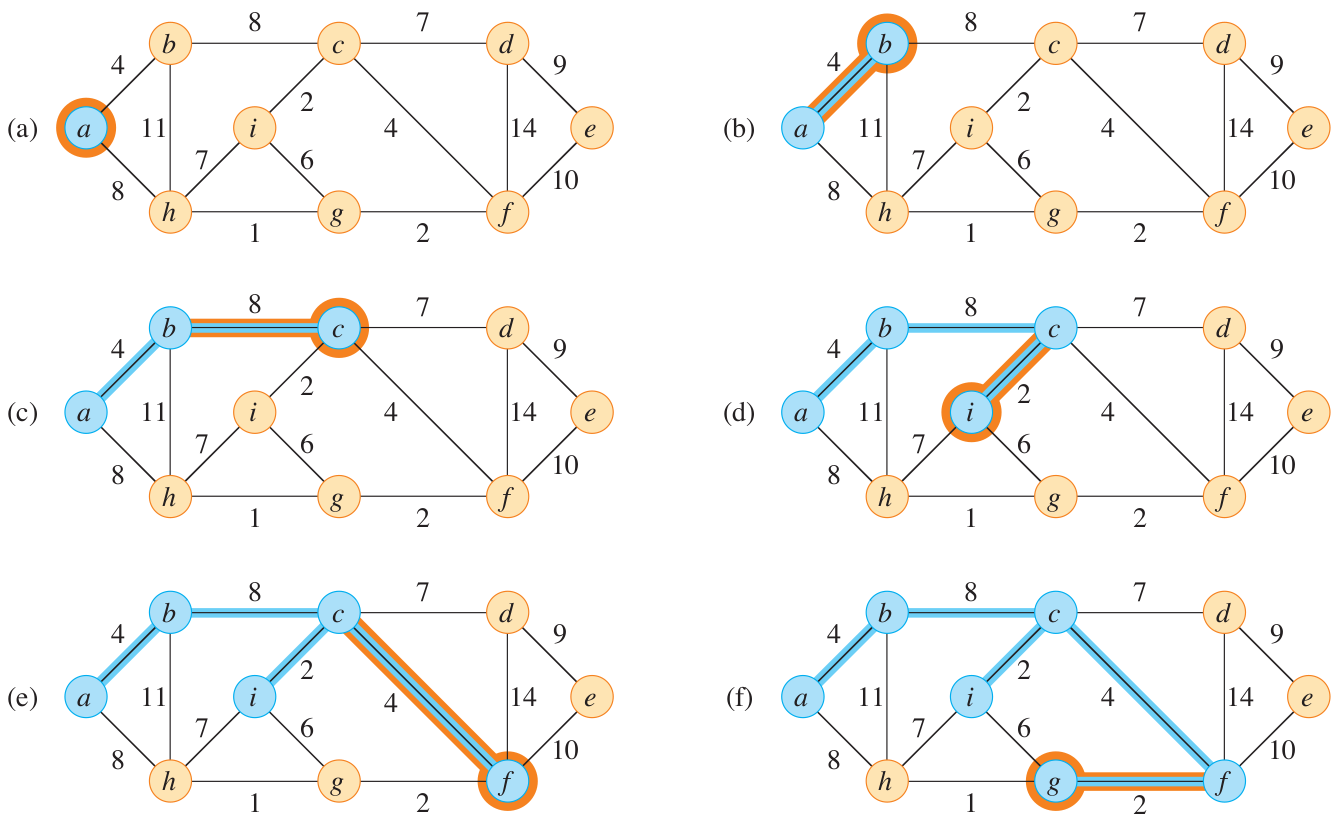
\includegraphics[width=0.6\textwidth]{figs/chap07/595-prim-1}
\end{figure}
\end{itemize}
\end{frame}

\begin{frame}{‌الگوریتم پریم}
\begin{itemize}\itemr
\item[-]
شکل زیر روند اجرای الگوریتم پریم را نشان می‌دهد.
\begin{figure}
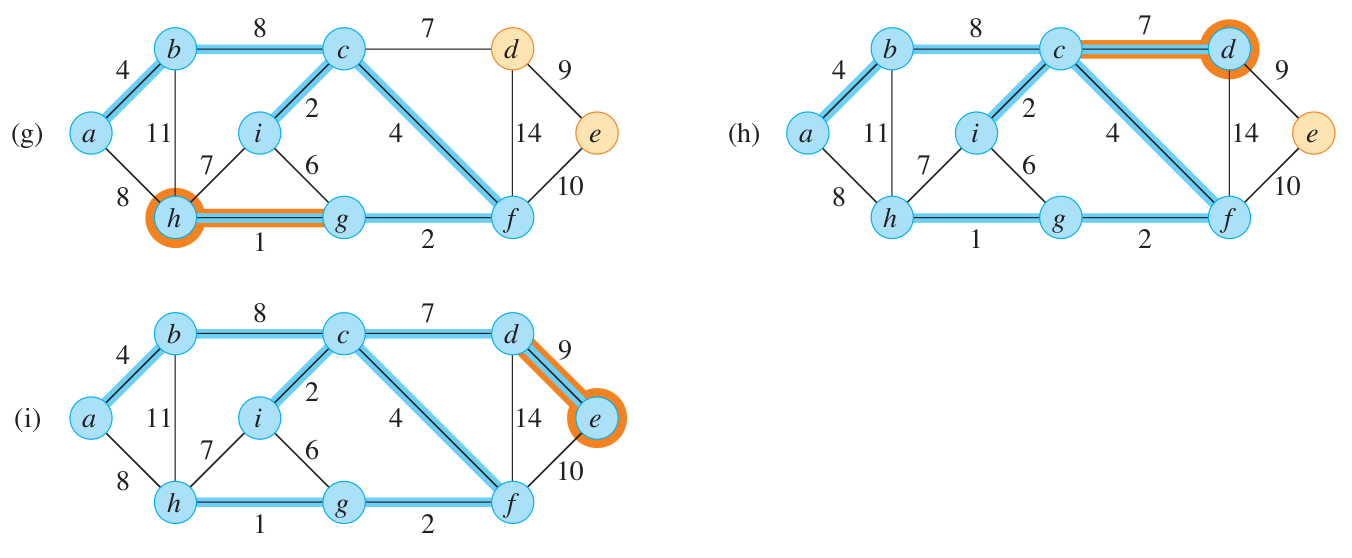
\includegraphics[width=0.6\textwidth]{figs/chap07/595-prim-2}
\end{figure}
\end{itemize}
\end{frame}

\begin{frame}{‌الگوریتم پریم}
\begin{itemize}\itemr
\item[-]
الگوریتم پریم در زیر نشان داده شده است.
\begin{algorithm}[H]\alglr
  \caption{Minimum Spanning Tree - Prim} 
  \begin{algorithmic}[1]
   \Func{Mst-Prim}{G,w,r}
   \For{each vertex u $\in$ G.V}
   		\State u.key = $\infty$
   		\State u.pred = Nil
   	\EndFor
   	\State r.key = 0
   	\State Q = $\emptyset$
   	\For{each vertex u $\in$ G.V}
   			\State Insert(Q,u)
   	\EndFor                    
  \end{algorithmic}
  \label{alg:merge}
\end{algorithm}
\end{itemize}
\end{frame}


\begin{frame}{‌الگوریتم پریم}
\begin{itemize}\itemr
\item[-]
\begin{algorithm}[H]\alglr
  \caption{Minimum Spanning Tree - Prim} 
  \begin{algorithmic}[1]
   \setcounter{ALG@line}{7}
   %\Func{Mst-Prim}{G,w,r}
   	\While{Q $\neq$ $\emptyset$}
   			\State u = Extract-Min(Q)		\LeftComment{add u to the tree}
   			\For{each vertex v in G.Adj[u]}		\LeftComment{update keys of u's non-tree neighbors}
   					\If{v $\in$ Q and w(u,v) < v.key}
   							\State v.pred = u
   							\State v.key = w(u,v)
   							\State Decrease-Key(Q,v,w(u,v))
   					\EndIf
   			\EndFor
   	\EndWhile                           
  \end{algorithmic}
  \label{alg:merge}
\end{algorithm}
\end{itemize}
\end{frame}


\begin{frame}{‌الگوریتم پریم}
\begin{itemize}\itemr
\item[-]
برای اضافه کردن یال جدید به درخت
\m{A}
، الگوریتم از صف اولویت
\m{Q}
استفاده می‌کند که در آن رئوسی که به درخت افزوده نشده‌اند نگهداری می‌شود.
\item[-]
برای هر رأس
\m{v}
، ویژگی
\m{v.key}
وزن کمینه یالی است که
\m{v}
را به یک رأس دیگر در درخت متصل می‌کند.
\item[-]
مقدار
\m{v.pred}
پدر رأس
\m{v}
را در درخت مشخص می‌کند.
\end{itemize}
\end{frame}


\iffalse
\begin{frame}{‌الگوریتم پریم}
\begin{itemize}\itemr
\item[-]
به طور ضمنی در این الگوریتم مجموعه
\m{A}
حاوی
\m{A = \{(v,v.pred) : v \in V-\{r\}-Q\}}
است.
\item[-]
وقتی الگوریتم به پایان می‌رسد، صف اولویت خالی می‌شود و در نتیجه داریم :
\begin{align*}
\m{A = \{(v,v.pred) : v \in V-\{r\}\}}
\end{align*}
\end{itemize}
\end{frame}
\fi



\begin{frame}{‌الگوریتم پریم}
\begin{itemize}\itemr
\item[-]
زمان اجرای الگوریتم پریم را به صورت زیر تحلیل می‌کنیم.
%به نحوه پیاده‌سازی صف اولویت بستگی دارد.
\item[-]
حلقهٔ
\code{while}
به تعداد
\m{|V|}
بار تکرار می‌شود و از آنجایی که عملیات
\code{Extract-Min}
در زمان
\m{O(lg|V|)}
اجرا می‌شود، زمان لازم برای انجام این عملیات
\m{O(|V|lg|V|)}
است.
\item[-]
حلقهٔ
\code{for}
در خطوط ۱۰ تا ۱۴ جمعاً
\m{O(|E|)}
بار تکرار می‌شود. هر فراخوانی
\code{Decrease-Key}
در زمان
\m{O(lg|V|)}
اجرا می‌شود، بنابراین الگوریتم پریم در زمان
\m{O(|V|lg|V|+|E|lg|V|)}
اجرا می‌شود. چون تعداد یال‌های گرافی که دارای درخت پوشای کمینه است، حداقل برابر با 
\m{|V|}
است، پس زمان اجرای الگوریتم پریم برابر با
\m{O(|E|lg|V|)}
 است.
\end{itemize}
\end{frame}

\iffalse
\begin{frame}{‌الگوریتم پریم}
\begin{itemize}\itemr
\item[-]
اگر صف اولویت با یک هرم فیبوناچی
\fn{1}{Fibonacci heap}
پیاده‌سازی شود، زمان اجرای الگوریتم پریم بهبود می‌یابد.
\item[-]
اگر هرم فیبوناچی تعداد
\m{|V|}
عنصر را نگهداری کند، تابع
\code{Exract-Min}
در زمان
\m{O(lgV)}
اجرا می‌شود و هریک از عملیات
\code{Insert}
و
\code{Decrease-Key}
در
\m{O(1)}
اجرا می‌شوند. بنابراین الگوریتم پریم می‌تواند در زمان
\m{O(E+VlgV)}
اجرا شود.
\end{itemize}
\end{frame}
\fi